\section{Theorie}
Röntgenstrahlung ist für das menschliche Auge nicht sichtbare Strahlung mit einer Wellenlänge unter 10 nm.
In einer Röntgenröhre entsteht Röntgenstrahlung durch zwei Prozesse bei der Beschleunigung von 
Elektronen von einer Kathode zu einer Anode in einem elektrischen Feld. 

Die Elektronen schlagen
beim Auftreffen auf die Anode Elektronen aus den inneren Schalen der Atome des Anodenmaterials heraus. 
Durch Übergänge von Elektronen höhrerer Energieniveaus werden Photonen entsprechend der 
freiwerdenen Bindungsenergie emittiert. Es entsteht ein Linienspektrum, welches charakteristisch für das 
Anodenmaterial ist, das charakteristische Röntgenspektrum. 

Röntgenstrahlung entsteht auch bei der Beschleunigung oder Abbremsung von Elektronen. Die 
Wellenlänge der so erzeugten Bremsstrahlung ist dabei abhängig von der Stärke der Beschleunigung oder 
Abbremsung und korrespondiert so zu der zwischen Kathode und Anode angelegten Beschleunigungsspannung.
Das Spektrum der Bremsstrahlung ist kontinuierlich und dem charakteristischen Spektrum überlagert.

\subsection*{Röntgenreflektivität an Grenzflächen}
Röntgenstrahlung hat einen Brechungsindex
\begin{equation*}
    n = 1 - \delta + i \beta
\end{equation*}
mit einem kleinen positiven Störungsparameter $\delta$ mit typischer Größenordnung 
$\delta \sim \mathcal{O}(10^{-6})$. Der Realteil $\text{Re}(n) = 1-\delta$ beschreibt die Brechung, der
Imaginärteil $\text{Im}(n) = \beta$ die Absorption.
Trifft eine elektromagnetische Welle auf eine Grenzfläche, so wird die Beziehung zwischen dem Winkel 
$\alpha_1$ der einfallenden Welle und dem Winkel $\alpha_2$ der transmittierten Welle durch das 
\textit{Snellius'sche Brechungsgesetz}
\begin{equation}
    n_1 \sin \alpha_1 = n_2 \sin \alpha_2 
    \label{eq:snellius}
\end{equation}
beschrieben. Bei Röntgenstrahlung wird der Realteil des Brechungsindex $n_2$ durch den Parameter $\delta$ 
kleiner als 1, sodass unterhalb eines kritischen Winkels $\alpha_\text{krit}$ das Snellius'sche Brechungsgesetz
\ref{eq:snellius} nicht mehr erfüllt werden kann und Totalreflektion auftritt.
Aus dem Snellius'schen Brechungsgesetz kann $\alpha_\text{krit}$ für Grenzflächen zwischen Vakuum und 
Materie berechnet werden. Es ergibt sich 
\begin{equation*}
    \alpha_\text{krit} = \sqrt{2 \delta}
\end{equation*}
unter Vernachlässigung von Absorption \cite{dissertation2}.

Die Brechung und Reflektion einer elektromagnetischen Welle an einer Grenzfläche wird durch die 
\textit{Fresnel'schen Formeln} über Transmissions- und Reflektionskoeffizienten $t$ und $r$ beschrieben. 
In den allgmeinen Gleichungen muss zwischen s- und p-Polarisation unterschieden werden, im Fall von 
Röntgenstrahlung ist diese Unterscheidung jedoch vernachlässigbar. Die Fresnel'schen Formeln sind dann 
\begin{align*}
    r &= \frac{n_1 \cos \alpha_1 - n_2 \cos \alpha_2}{n_1 \cos \alpha_1 + n_2 \cos \alpha_2} \\
    t &= \frac{2 n_1 \cos \alpha_1}{n_1 \cos \alpha_1 + n_2 \cos \alpha_2} \, .
\end{align*}
Die Fresnelreflektivität berechnet sich über den Reflektionskoeffizienten $r$ durch $R_F = |r|^2$.
Für Einfallswinkel $\alpha_1 < 3 \alpha_\text{krit}$ kann die Fresnelreflektivität genähert werden zu \cite{dissertation3}
\begin{equation*}
    R_F = \left(\frac{\alpha_\text{krit}}{2 \alpha_1}\right)^4 \, .
\end{equation*}

\subsection*{Kiessig-Oszillationen und Parratt-Algorithmus}
Besteht das zu untersuchende Medium aus mehreren Schichten, treten \textit{Kiessig-Oszillationen} auf, siehe Abb. \ref{fig:kiessig}. 
\begin{figure}
    \centering
    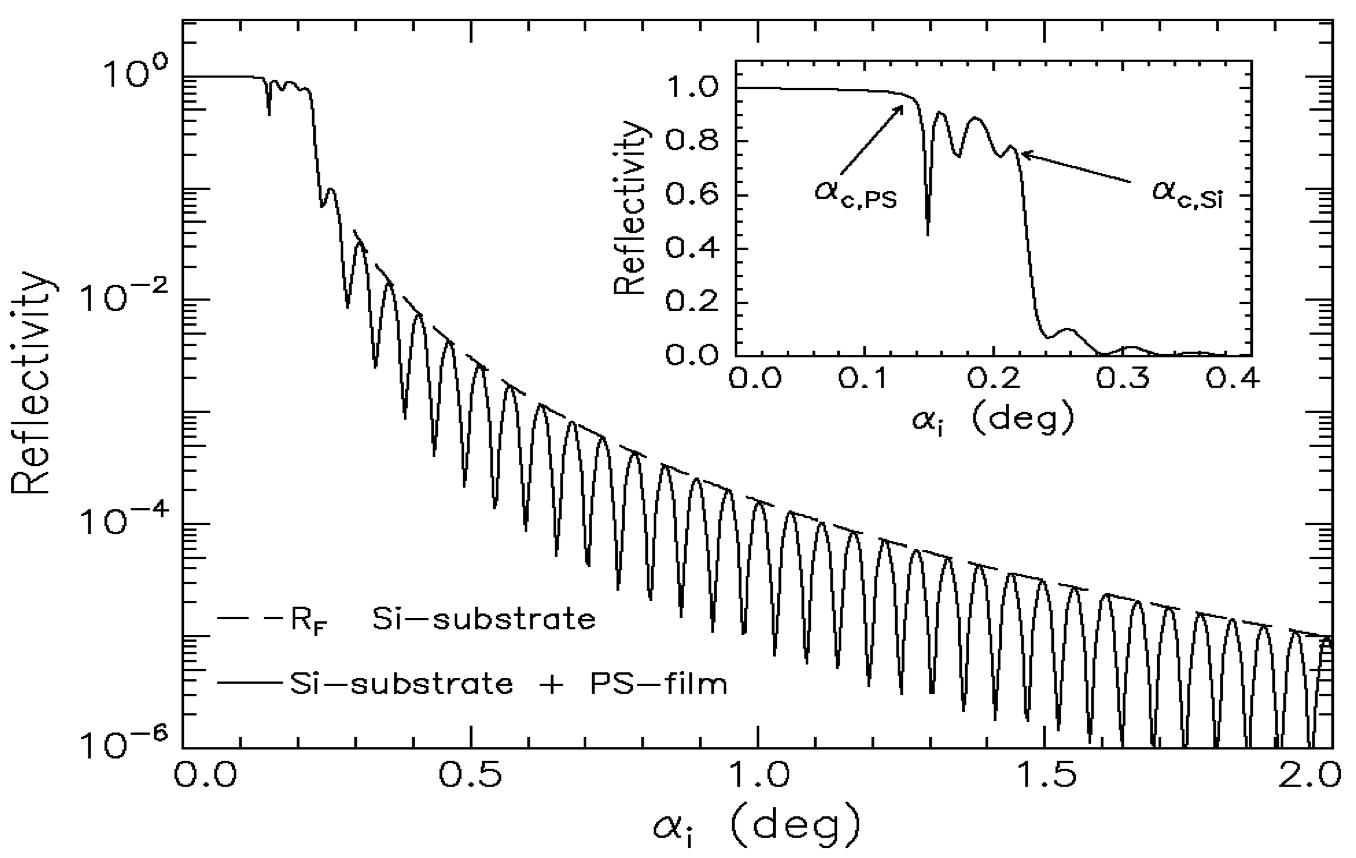
\includegraphics[width = \linewidth]{kiessig.png}
    \caption{Berechnete Röntgenreflektivität $R$ einer Polystyrol-Schicht mit Dicke $d = 800$ Å auf einem Siliziumsubstrat in 
    Abhängigkeit des Einfallswinkels $\alpha_i$ bei $\lambda = 1,54$ Å (Durchgezogene Linie) sowie 
    Fresnelreflektivität des Substrats (Gestrichelte Linie) \cite{kiessig}.}
    \label{fig:kiessig}
\end{figure}
Diese Oszillationen der Reflektivität entstehen durch Interferenz. An jeder Schicht im Medium wird die 
beim vorherigen Brechungsporzess transmittierte Welle gebrochen, die dabei reflektierten Wellen 
interferieren. Aus der Lage der Oszillationsmaxima bei konstruktiver Interferenz, die auftritt, wenn der 
Gangunterschied zwischen zwei interferierenden Wellen
ein gerades Vielfaches der halben Wellenlänge beträgt, kann für ein System aus zwei Schichten über
\begin{equation*}
    d = \frac{2 \pi}{\Delta q} \approx \frac{\lambda}{2 \Delta \alpha_1}
\end{equation*} 
mit dem Abstand der zwei Maxima $q = 2 k \sin \alpha_1 = \frac{4 \pi}{\lambda} \sin \alpha_1$
und der Periode $\Delta \alpha_1$ die Schichtdicke $d$ bestimmt werden \cite{dissertation}, siehe Abb. \ref{fig:schichtdicke}.
\begin{figure}
    \centering
    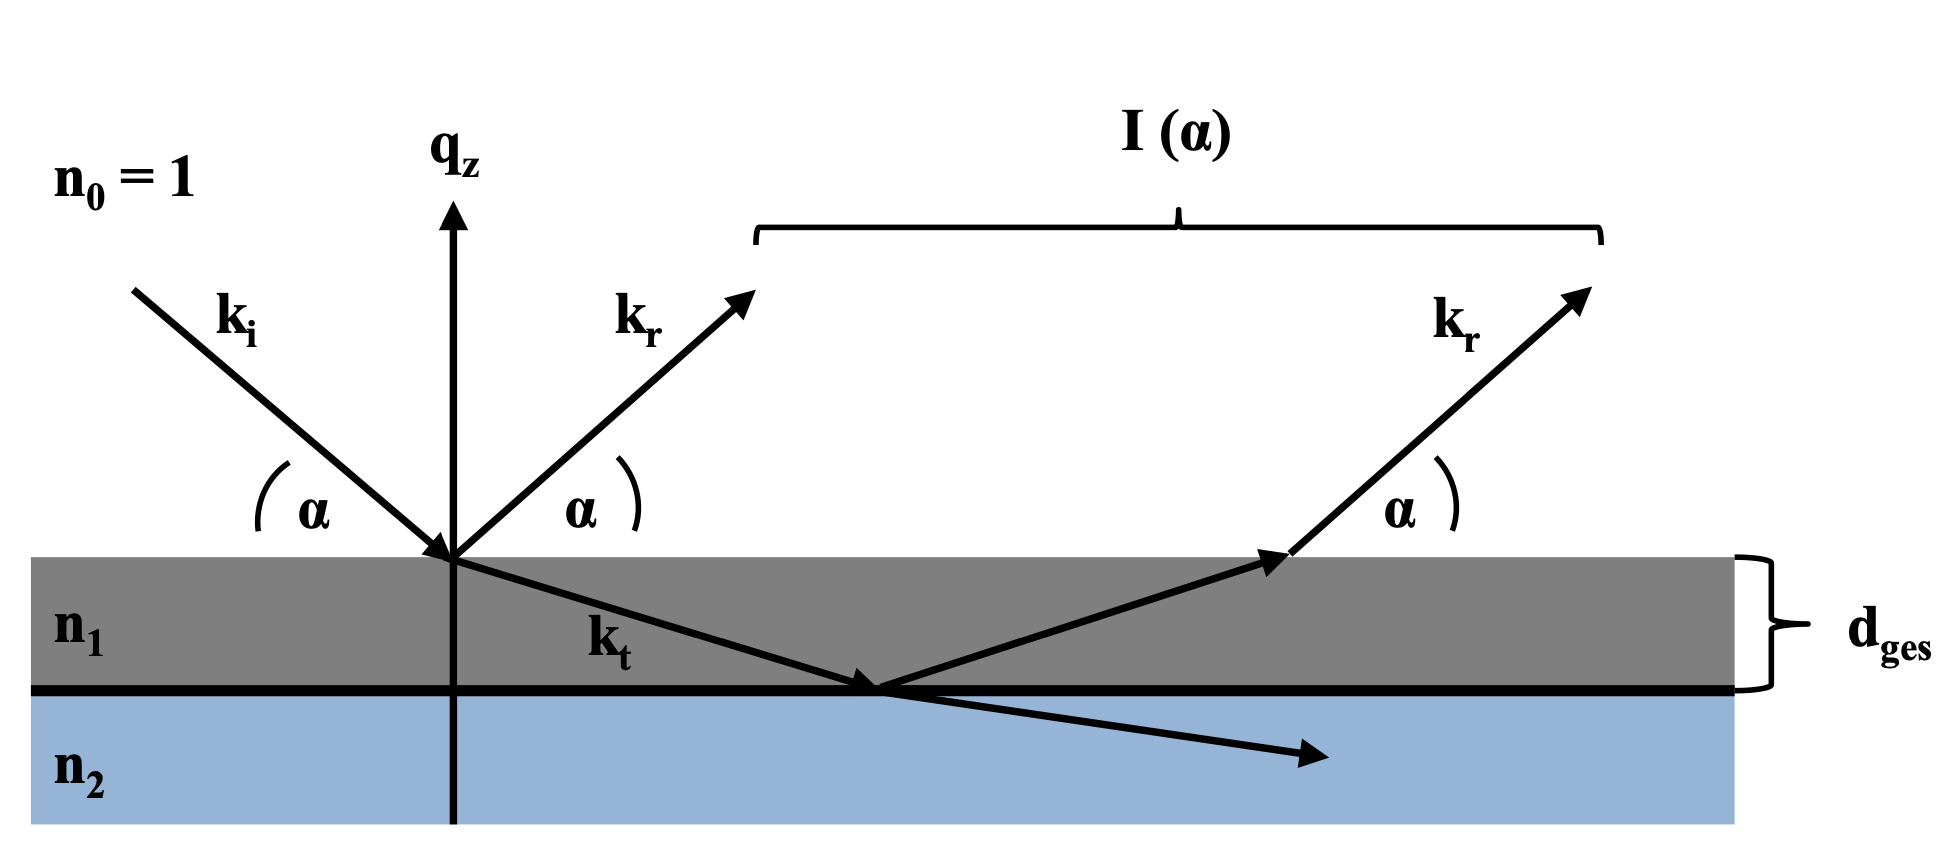
\includegraphics[width = \linewidth]{schichtdicke.png}
    \caption{Streugeometrie an einen Zwei-Schicht-System mit $n_0 < n_1 < n_2$. Kiessig-Oszillationen 
    mit Intensität $I(\alpha)$ entstehen durch konstruktive Interferenz der Reflektionen \cite{dissertation}.}
    \label{fig:schichtdicke}
\end{figure}
Bei einem System mit mehr als zwei Schichten überlagern sich verschiedene Oszillationen. Mit dem \textit{Parratt-Algorithmus}
kann die Reflektivität eines Mehrschichtsystems über die Fresnel'schen Formeln rekursiv bestimmt werden.
Die Rekursionsgleichung beschreibt das Amplitudenverhältnis der reflektierten und transmittierten Strahlung
zwischen den Schichten $j$ und $j+1$. 
\begin{align}
    X_j = \frac{R_j}{T_j} &= e^{-2 i k_{z,j}z_j} \cdot \frac{r_{j, j+1} + X_{j+1}e^{2 i k_{z,j+1}z_j}}{1+r_{j, j+1} + X_{j+1}e^{2 i k_{z,j+1}z_j}} \\
    r_{j, j+1} &= \frac{k_{z,j}-k_{z, j+1}}{k_{z,j}+k_{z, j+1}}
\end{align}
mit der Koordinate $z_j$, die die Lage der $j$-ten Grenzfläche beschreibt und der Fresnelreflektivität
der $j$-ten Grenzfläche $r_{j, j+1}$.
Aufgrund der geringen Eindringtiefe von Röntgenstrahlung wird angenommen, dass an der untersten Schicht 
keine Transmission mehr stattfindet.
Die Berechnung eines Systems aus $n$ Schichten beginnt bei $R_{n+1} = 0$, sodass sukessiv die $X_j$ bis zur 
letzten Grenzfläche berechnet werden können. 
Bei rauen Schichten mit einer Rauheit $\sigma$, die kleiner ist als die Schichtdicke, kann der Parratt-Algorithmus
mit modifizierten Fresnelkoeffizienten verwendet werden. Dann gilt \cite{dissertation}
\begin{equation}
    r_{j, j+1}^\text{rau} = e^{-2 i k_{z,j} k_{z, j+1} \sigma_j^2} \cdot \frac{k_{z,j}-k_{z, j+1}}{k_{z,j}+k_{z, j+1}} \, .
\end{equation}

\subsection*{Geometriefaktor und Geometriewinkel}
Bei der Untersuchung von Oberflächen mit Röntgenreflektometrie muss berücksichtigt werden, dass der 
Röntgenstrahl erst ab einem hinreichend großen Einfallswinkel vollständig auf die Probenoberfläche trifft.
Bei sehr kleinen Einfallswinkels ist die vom Röntgenstrahl getroffene Fläche größer als die Probenoberfläche,
sodass nicht die gesamte einfallende Strahlung reflektiert wird. Dies zeigt sich in einem Abfall der 
Reflektivität im Bereich sehr kleiner Einfallswinkel.
Dieser Geometriewinkel $\alpha_g$ wird im Geometriefaktor $G$ berücksichtigt. Dieser ist mit dem Durchmesser 
$D$ der Probenoberfläche für Einfallswinkel $\alpha_i < \alpha_g$ definiert als 
das Verhältnis aus Strahlbreite $D \sin \alpha_i$, das die die Probenoberfläche trifft, und 
Gesamtstrahlbreite $d_0$ und gegeben durch
\begin{equation}
    G = \frac{D}{d_0} \sin \alpha_i = 1 \, .
    \label{eq:geometrie}
\end{equation}
